\chapter{評価実験}
本研究で実装した検知システムにおける定常的な動作負荷の評価を行い,DDoS攻撃を行うマルウェアを用いて検知精度の評価を行った.

\section{システムコール呼び出し履歴を用いた検知手法による定常的な動作負荷の評価}

IoTデバイスにマルウェアが動作していない状況下において,提案した検知システムによるマルウェア探索動作によってIoTデバイス本来の動作が阻害されていないことを評価するために,3.4節で述べたように,LinuxOSを対象とする既存のアンチウィルスソフトであるClam AVを動作させた状態のCPU,メモリの使用率を基準値とし,提案した検知システムによってMiraiが動作していない状況での,CPU,メモリの使用率についてsarコマンドを用いて1分間計測を行った.
sarコマンドを用いて得たCPU,メモリの使用率について,Clam AVと比較を行った結果が図\ref{fig:strace_cpu},\ref{fig:strace_mem}になる.ClamAVを動作させた状態のIoTデバイスのCPU使用率,メモリ使用率の値は3.4節で計測したデータを用いた.
 
\begin{figure}[h]
    \centering
       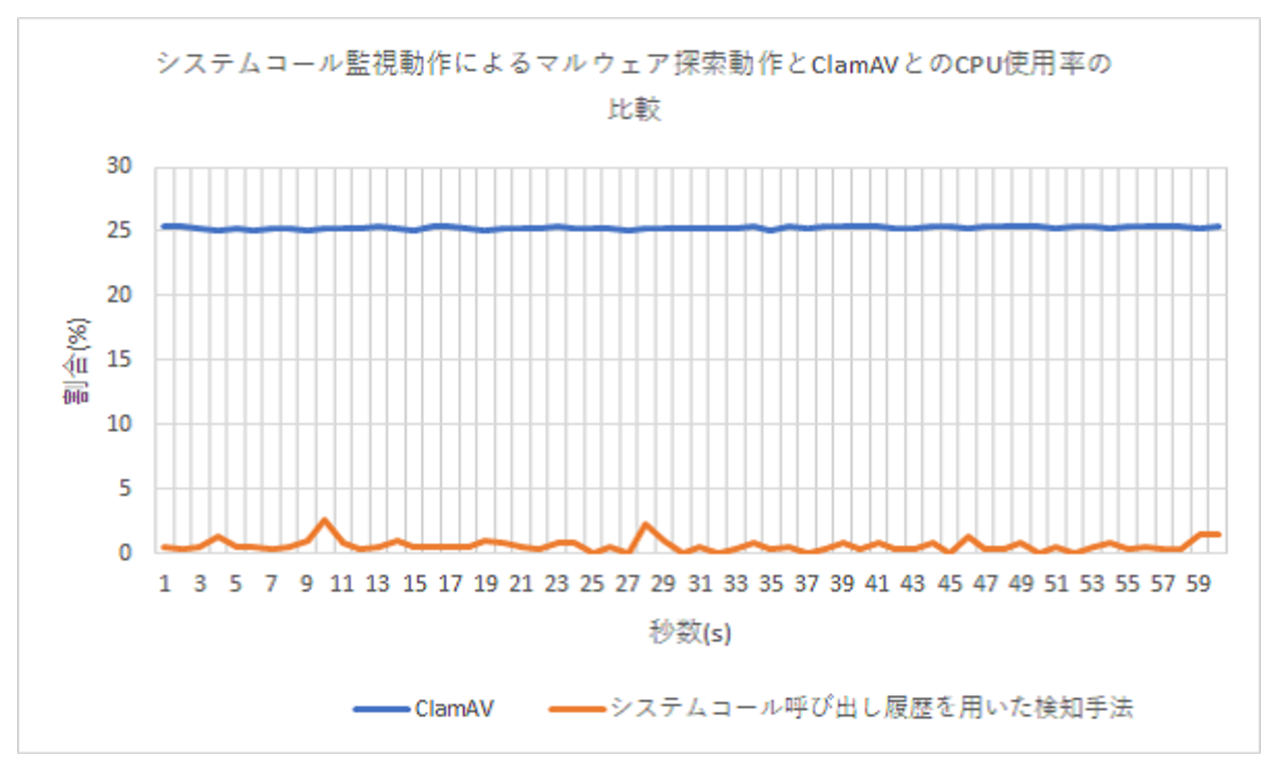
\includegraphics[width=120mm]{figures/strace_cpu.eps}
    \caption{システムコール呼び出し履歴によるマルウェア探索動作とClamAVとのCPU使用率の比較}
        \label{fig:strace_cpu}
\end{figure}
  
\begin{figure}[h]
        \centering
           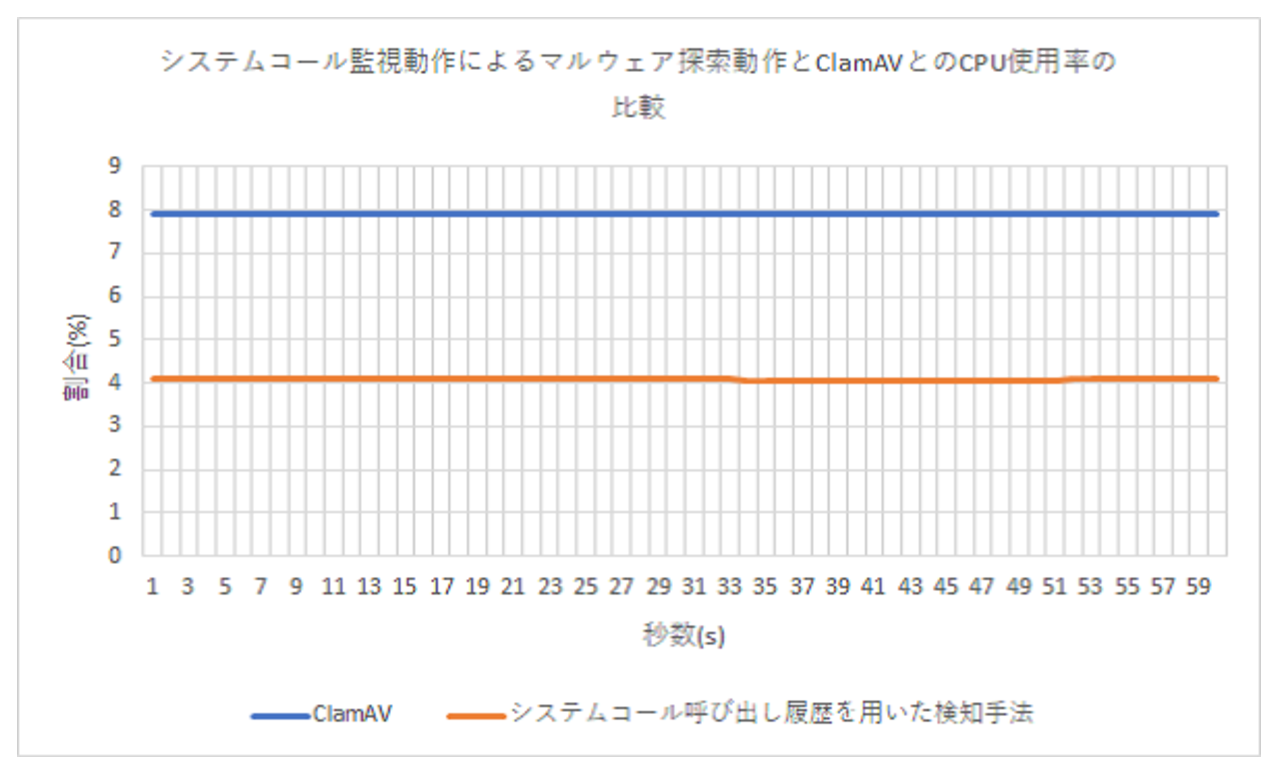
\includegraphics[width=120mm]{figures/strace_mem.eps}
        \caption{IoTデバイス上でマルウェアが動作していない状況におけるマルウェア探索のメモリ使用率}
        \label{fig:strace_mem}
\end{figure}

   
 Clam AntiVirusを利用した場合には,平均CPU使用率が24.27\%,メモリ使用率は7.92\%であり.提案した検知手法では,平均CPU使用率が0.57\%,メモリ使用率が4.08\%となった.メモリ使用率は比較対象のClam AntiVirusと提案した検知手法では97.6\%減,CPU使用率は,Clam AntiVirusに対して提案した検知手法は48.4\%減となった.


\section{Miraiとその亜種マルウェアを対象とする判別性能評価}
ハニーポットを用いてDDoS攻撃を行うマルウェアを収集し,収集したマルウェアを検体として用いて,システムコール呼び出し履歴を用いた検知手法の検知精度の評価を行った.

\subsection{ハニーポットによるマルウェアの収集}
ハニーポットと呼ばれる攻撃者に端末を意図的に侵入させ,マルウェアをダウンロードさせ実行するまでの挙動を取得するシステムを用いてDDoS攻撃を行うマルウェアを収集した.シェルの対話の中でダウンロードされるバイナリファイルを実行させることなく保存することが可能なMichel Oosterhofによって開発されたCowrie\cite{Cowrie}と呼ばれるハニーポットを用いた.Cowrieによって収集されたバイナリファイルについてVirus Totalと呼ばれるマルウェア検知オンラインサービスを用いて解析を行い,DDoS攻撃を行うマルウェアの分類分けを行った.Virus Total\cite{Virus}はユーザーから投稿された検体を54のウィルス対策エンジンによって解析するオンラインサービスであり,投稿された検体についてマルウェアの分類を知ることができる.2019/01/09から2019/01/28の期間でハニーポットを断続的に運用してバイナリファイルの収集を行った.収集したバイナリファイルをVirus Totalに投稿し,Virus Totalの解析結果から,MiraiまたはMiraiの亜種のマルウェアをDDoS攻撃を行うマルウェアとして分類分けした.分析した結果,収集したバイナリファイルは,空ファイルのものや,マルウェアをダウンロードさせ実行させるファイル,DDoS攻撃を行うマルウェアのバイナリファイル等が散見され,DDoS攻撃を行うマルウェアは57検体が存在し,マルウェアの実行可能な検体は49検体であった.

\subsection{提案システムによるマルウェアの検知精度評価}
前項で収集した49検体のDDoS攻撃を行うマルウェアを用いてシステムコール呼び出し履歴を用いた検知手法の検知精度の評価を行った.入手したマルウェアをネットワークから隔離した状態で検知システムを動作させマルウェアの検知できるか評価を行った.正規プログラムは,Linuxに標準でインストールされているプログラムの44検体を利用した.実験の評価指数として,Accuracy,TPR(True Positive Rate),TNR(True Negative Rate),FPR(False Positive Rate),FNR(False Negative Rate)を用いる.Accuracyは,マルウェアを正しく判別できた割合である.TPRはマルウェアをマルウェアと判別できた割合,TNRは正規プログラムを正規プログラムと判別した割合,FPRはマルウェアを正規プログラムと判別した割合,FPRは正規プログラムをマルウェアとして判別した割合である.Accuracy,TPR,TNR,FPR,FNRを下記の式で算出する.

\begin{eqnarray}
    Accuracy & = & \frac{正しくマルウェアと判別された検体数}{検体の総数}\\
    TPR & = & \frac{マルウェア検体がマルウェアと判別された検体数}{マルウェア検体の総数}\\
    TNR & = & \frac{正規プログラムを正規プログラムとして判別された検体数}{正規プログラムの総数}\\
    FNR & = & \frac{マルウェア検体が正規プログラムとして判別された検体数}{マルウェア検体の総数}\\ 
    FPR & = & \frac{正規プログラムをマルウェアとして判別された検体数}{正規プログラムの総数}
\end{eqnarray}

提案システムによるプログラムの判別結果を表\ref{tab:detect}に示し,Accuracy,TPR,TNR,FPR,FNRの結果を表\ref{tab:result}に示す.

\newpage 

\begin{table}[h]
    \centering
    \caption{提案システムによるマルウェア判別結果}
    \label{tab:detect}
\begin{tabular}[t]{lccc}
    \hline
            &  &  \multicolumn{2}{c}{判別結果}  \\ \hline
            &  &  マルウェア & 正規プログラム \\ \hline 
            真の結果 & マルウェア & 41 & 8 \\ \hline
            & 正規プログラム & 0 & 44 \\ \hline
\end{tabular}
\end{table}

\begin{table}[h]
     \caption{プログラムの判別結果} 
     \label{tab:result}
     \centering 
    \begin{tabular}{|c|c|c|c|c|} \hline 
    Accuracy & TPR    & TNR     & FNR    & FPR   \\ \hline
    91.3\%   & 83.4\% & 100.0\% & 16.6\% & 0.0\% \\ \hline
    \end{tabular}
\end{table}

評価の結果,Accuaryは91.3\%と高い精度となっており,TPRの値が,83.4\%であり,FPRの値が0\%である.TPRが83.4\%のため,Mirai亜種の多くのマルウェアは作成されたMiraiのスキャン機能をそのまま流用している場合が多いことがわかった.しかし,スキャン活動を行っている一部のマルウェアを提案システムによって検出することができなかった.検出ができなかった要因としてスキャン活動を行っていない場合とスキャン活動を行っている際にスキャンしているportが23ではなく,他のportをスキャンしてため,検知条件に一致しなかったためである.TNRが高い精度を示した理由が,対象となっている正規プログラムがLinuxに標準でインストールされているプログラムを利用している事が挙げられる.そのため,組織や,個人で作成されたプログラムでは誤検知をする可能性がある.